\chapter{Opis projektnog zadatka}
		
		
		Cilj je ovog zadatka napraviti aplikacijsko programsko sučelje koje će olakšati komunikaciju između istraživača, voditelja postaje te tragača u akcijama praćenja divljih životinja.
		
		Prvi korak za korištenje aplikacije je registracija. Prilikom registracije korisnik odabire koju ulogu će imati u aplikaciji. On može biti istraživač, voditelj postaje ili tragač.
		Podaci koje je potrebno unijeti pri registraciji su sljedeći:
		\begin{packed_item}
			\item \textit{korisničko ime}
			\item \textit{fotografija}
			\item \textit{lozinka}
			\item \textit{ime}
			\item \textit{prezime}
			\item \textit{email adresa.}
		\end{packed_item}
		
		Registracija završava potvrdom preko emaila, te dodatno voditelja i istraživača treba potvrditi administrator. Sličan primjer obrasca za registraciju prikazan je u nastavku na slici 2.1.
		
		\begin{figure}[H]
			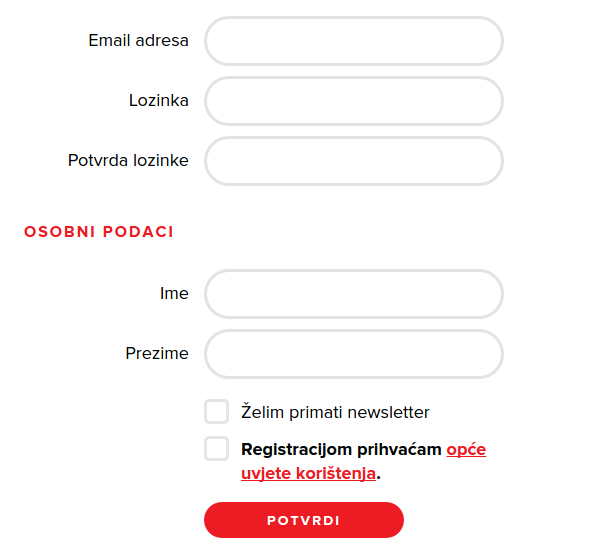
\includegraphics[scale=0.55]{slike/probrazac.PNG} %veličina u odnosu na širinu linije
			\centering
			\caption{Primjer obrasca za registraciju}
			\label{fig:probrasca} %label mora biti drugaciji za svaku sliku
		\end{figure}
		
		
		
		\textbf{Voditelj} vodi svoju postaju koja ima naziv po području na kojem se nalazi (npr. Kopački rit, Velebit…). Također posjeduje popis \textbf{tragača} koji su dio njegove postaje te na koji način mogu obavljati istraživanje. Mogućnosti kretanja tragača su sljedeće:
		\begin{packed_item}
			\item \textit{pješke}
			\item \textit{automobilom}
			\item \textit{cross motorom}
			\item \textit{brodom}
			\item \textit{dronom}
			\item \textit{helikopterom.}
		\end{packed_item}
		
		Akcija kreće tako što \textbf{istraživač} izda zahtjev za novom akcijom te od voditelja postaje traži da pošalje kvalificirane tragače. Istraživač preko karte koja mu se prikazuje može zadati zadatke svim tragačima na akciji. Tragač se može maknuti s akcije nakon što izvrši sve zadatke koji su mu zadani.
		
		Zadaci su da tragač prođe određenom rutom te dođe do neke lokacije i postavi kameru ili gps uređaj. Na nekoj akciji istraživač i tragač mogu ostaviti komentar na karti.
		
		Cilj svih akcija je pratiti životinje te odrediti povijest njihovog kretanja zbog čega sve praćene životinje imaju gps uređaj. Praćene životinje imaju sljedeće podatke:
		\begin{packed_item}
			\item \textit{naziv vrste}
			\item \textit{slika}
			\item \textit{opis.}
		\end{packed_item}
		
		Sve karte koje se prikazuju su toplinske karte (eng. \textit{heatmaps}). Primjer jedne takve toplinske karte je u nastavku na slici 2.2.
		
		\begin{figure}[H]
			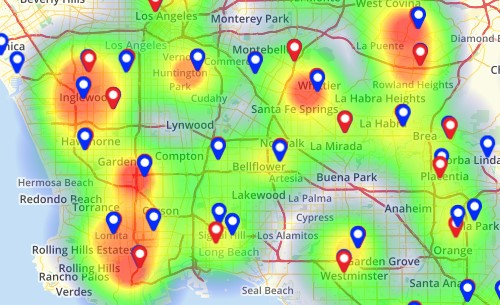
\includegraphics[scale=0.8]{slike/heatmap.JPG} %veličina u odnosu na širinu linije
			\centering
			\caption{Primjer toplinske karte}
			\label{fig:prkarte} %label mora biti drugaciji za svaku sliku
		\end{figure}
		
		Istraživač može izabrati koja će mu se karta prikazati. Može pregledavati karte s podacima o praćenim životinjama:
		\begin{packed_item}
			\item \textit{povijesne pozicije svih praćenih životinja }
			\item \textit{trenutne pozicije svih praćenih životinja.}
		\end{packed_item}
		
		Dodatna stavka koju treba odabrati je želi li podatke o određenoj jedinki ili o svim životinjama neke vrste. 
		
		Osim toga, ima pristup kartama s podacima o tragačima. Karte koje može pregledavati sadržavaju sljedeće podatke:
		\begin{packed_item}
			\item \textit{povijesne pozicije svih tragača na jednoj akciji}
			\item \textit{trenutne pozicije svih aktivnih tragača na jednoj akciji.}
		\end{packed_item}
		
		Tragače koje želi imati prikazane na karti treba odabrati po tipu prijevoza ili može pregledavati pozicije pojedinačnih tragača.
		
		Također, pristup karti trenutne akcije u kojoj je sudionik ima i tragač.
		Na njegovoj su karti vidljivi sljedeći podaci:
		\begin{packed_item}
			\item \textit{zadaci koje on treba obaviti}
			\item \textit{trenutna pozicija ostalih aktivnih tragača na toj akciji}
			\item \textit{trenutna pozicija praćenih životinja.}
		\end{packed_item}
		
		Pronašli smo nekoliko aplikacija koje imaju sličnu ulogu kao naša te su navedene u nastavku.
		
		Aplikacija \textit{eWildLife} je aplikacija s geooznakama za praćenje divljih životinja, slučajeve ubijanja istih te sukobe čovjeka i životinja te životinja međusobno. U nastavku na slici 2.3. prikazana je stranica za unošenje novih sukoba u ovoj aplikaciji.
		
		\begin{figure}[H]
			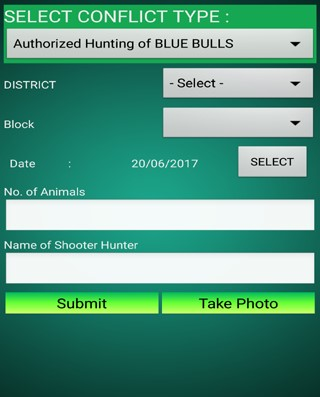
\includegraphics[scale=0.75]{slike/primjera1.JPG} %veličina u odnosu na širinu linije
			\centering
			\caption{Aplikacija eWildLife}
			\label{fig:ewildlife} %label mora biti drugaciji za svaku sliku
		\end{figure}
		
		Aplikacija \textit{Kwibi} bavi se sličnom problematikom kao prethodno navedena aplikacija, rješava probleme sukoba između ljudi i divljih životinja. Ova aplikacija koristi kartu, što je slično kao i u našoj aplikaciji, a njihov je primjer u nastavku na slici 2.4.
		
		\begin{figure}[H]
			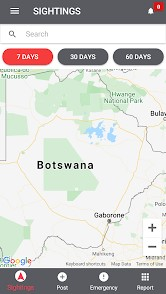
\includegraphics[scale=0.75]{slike/primjera2.JPG} %veličina u odnosu na širinu linije
			\centering
			\caption{Aplikacija Kwibi}
			\label{fig:kwibi} %label mora biti drugaciji za svaku sliku
		\end{figure}
		
		Sljedeća je aplikacija \textit{IMammalia} koja je pokrenuta u sklopu projekta MammalNet diljem Europe, a između ostalog i na Agronomskom fakultetu u Zagrebu. Na stranicu se može registrirati kao tragač ili osmatrač. Tragači u aplikaciju postavljaju fotografije divljih životinja sa svojih kamera koje osmatrači mogu pregledavati i kategorizirati. U nastavku je primjer jedne takve fotografije na slici 2.5.
		
		\begin{figure}[H]
			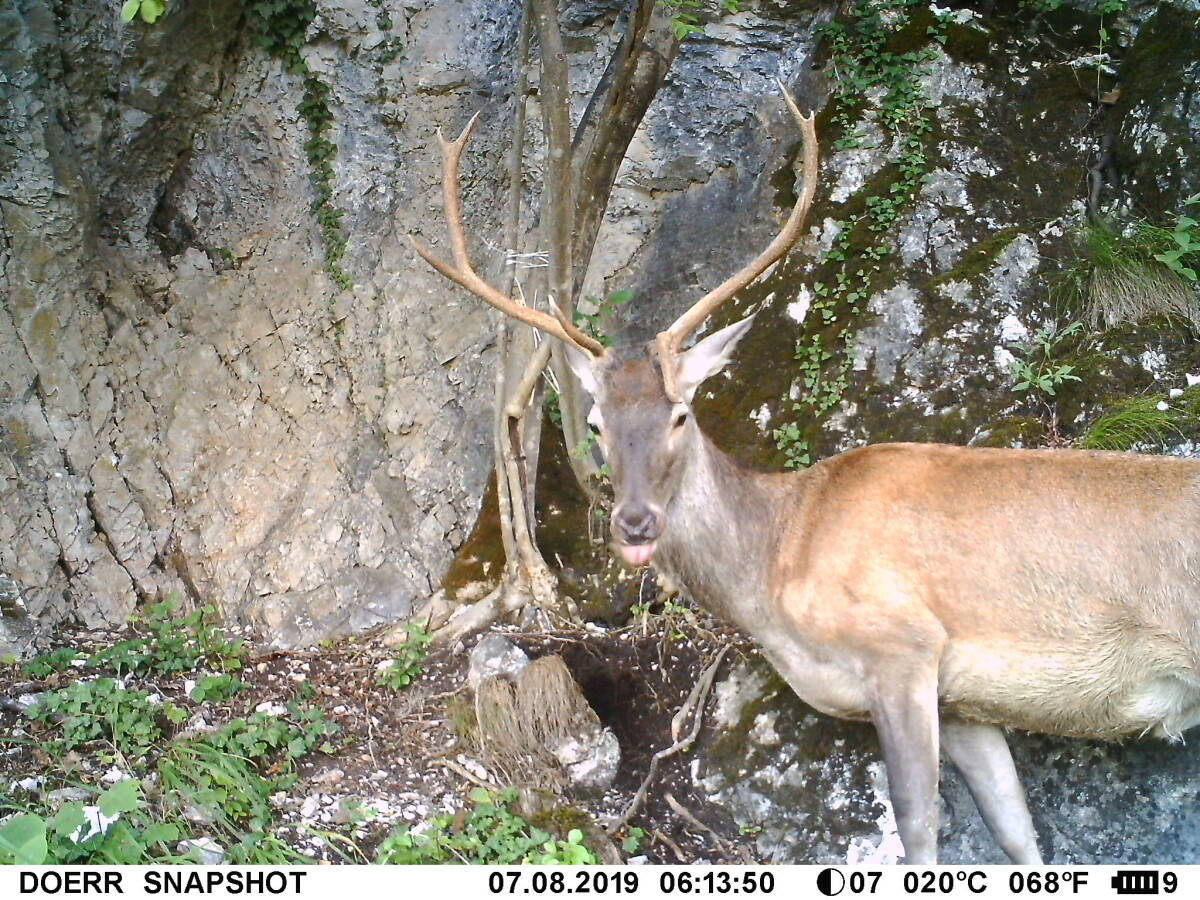
\includegraphics[scale=0.75]{slike/primjera3.JPG} %veličina u odnosu na širinu linije
			\centering
			\caption{Aplikacija IMammalia}
			\label{fig:mammal} %label mora biti drugaciji za svaku sliku
		\end{figure}
		
		Naša aplikacija razlikuje se od ostalih po tome što jedina nudi organizaciju cjelovitog istraživanja i jednostavnu komunikaciju između korisnika (voditelj postaje, istraživač, tragači), dok su ostale aplikacije fokusirane na sukobe između ljudi i životinja te kategorizaciju životinja.
		
		Neke od ideja koje je naš tim smislio, a mogle bi u budućnosti unaprijediti aplikaciju kao što je naša su sljedeće:
		\begin{packed_item}
			\item \textit{prikazane male ikonice životinja na karti}
			\item \textit{klikom na životinju otvara se detaljan opis i fotografija vrste}
			\item \textit{svijetli i tamni način rada}
			\item \textit{algoritam za automatsko slanje najkompatibilnijih tragača na akciju, bez posredovanja voditelja postaje.}
		\end{packed_item}
		
		
		
	